\def\CTeXPreproc{Created by ctex v0.2.9, don't edit!}
%\documentclass{beamer}
\documentclass[%handout,
xcolor=pdftex]{beamer}
\mode<presentation> {
  \usetheme{Warsaw}
  \setbeamercovered{transparent}
}
\let\Tiny=\tiny
\usetheme{Singapore}
\usecolortheme{dolphin}
\usepackage{amsmath}
\usepackage{textcomp}
\usepackage{amssymb}
\usepackage{amsthm}
\usepackage{graphicx}
\usepackage{color}
\usepackage{lipsum}
\usepackage{hyperref}
\usepackage{multirow}
\usepackage{bm}
\DeclareMathSymbol{\Phi}{\mathalpha}{operators}{8}
%\setbeamertemplate{headline}{}
\setbeamertemplate{footline}[page number]
\newcommand\Fontvi{\fontsize{9pt}{8}\selectfont}
\newcommand\Fontvii{\fontsize{7pt}{8}\selectfont}
\newcommand{\backupbegin}{
   \newcounter{finalframe}
   \setcounter{finalframe}{\value{framenumber}}
}
\newcommand{\backupend}{
   \setcounter{framenumber}{\value{finalframe}}
}\newtheorem{proposition}{Proposition}
\title{Unit 23: Regression with ARMA Errors}
\author[STAT 5170: Applied Time Series, Unit 25]{Taylor R. Brown}
\institute{Department of Statistics, University of Virginia}
\date{Fall 2020}

\AtBeginSubsection[] {
  \begin{frame}<beamer>{Outline}
    \tableofcontents[currentsection,currentsubsection]
  \end{frame}
}



\begin{document}


\frame{\titlepage}


\begin{frame}
\frametitle{Readings for Unit 23}

Textbook chapter 3.8.

\end{frame}


\begin{frame}
\frametitle{Last Unit}
\begin{enumerate}
\item Linear filters to enhance/retain or dampen certain frequencies.
\end{enumerate}
\end{frame}

\begin{frame}
\frametitle{Motivation}

One way to explore the relationship between two time series is via regression. One of the assumptions in linear regression is that the errors are independent. With time series, the errors are unlikely to be independent.


\end{frame}

\section{Regression Model with Correlated Errors}
\frame{\tableofcontents[currentsection]}

\begin{frame}
\frametitle{Regression Model with Correlated Errors}

In linear regression, the error terms are assumed to be i.i.d. $N(0, \sigma_w^2)$.

\vspace{10mm}

\textbf{Question}: What is a consequence if the errors are not independent?

\vspace{10mm}

We will see how we can adjust the linear regression model to allow for correlated errors.

\end{frame}

\begin{frame}
\frametitle{Regression Model with Correlated Errors}

Consider the classical regression model:

\begin{equation} \label{eq:classic}
y_t = \sum_{j=1}^r \beta_j z_{tj} + x_t
\end{equation}

where

\begin{itemize}
\item $y_t$: response variable at time $t$,
\item $z_{tj}$: the $j$th predictor at time $t$,
\item $\beta_j$: the $j$th coefficient,
\item $x_t$: error term that is Gaussian white noise.
\end{itemize}

\end{frame}



\begin{frame}
\frametitle{Regression Model with Correlated Errors}

Using matrix and vector notation, (\ref{eq:classic}) can be written as

\begin{equation} \label{eq:matrix}
\boldsymbol{y} = \boldsymbol{Z \beta} + \boldsymbol{x}
\end{equation}

where

\begin{itemize}
\item $\boldsymbol{y} = (y_1, \cdots, y_n)^\prime$,
\item $\boldsymbol{Z}$ is the $n \times r$ design matrix,
\item $\boldsymbol{\beta} = (\beta_1, \cdots, \beta_r)^\prime$,
\item $\boldsymbol{x} = (x_1, \cdots, x_n)^\prime$
\item $\text{Var}(\boldsymbol{x}) = \{\gamma_x(s,t) \}_{s,t} = \Gamma$
\end{itemize}

\end{frame}

\begin{frame}
\frametitle{Regression Model with Correlated Errors}

\begin{itemize}
\item In (\ref{eq:classic}) and (\ref{eq:matrix}), ordinary least squares (OLS) regression is used to estimate the coefficients.
\item If $x_t$ are correlated with some covariance $\gamma_x$, then \textbf{weighted} least squares (WLS) should be used instead.
\end{itemize}


\end{frame}

\begin{frame}
\frametitle{Weighted Least Squares}

Let $\boldsymbol{\Gamma}$ denote the covariance matrix for $\boldsymbol{x}$, then multiplying (\ref{eq:matrix}) by $\boldsymbol{\Gamma}^{-1/2}$, we obtain\\

\vspace{15mm}

\begin{equation} \label{eq:matrix2}
\boldsymbol{y^*} = \boldsymbol{Z^* \beta} + \boldsymbol{\delta}
\end{equation}

where

\vspace{30mm}

\end{frame}

\begin{frame}
\frametitle{Weighted Least Squares}

So (\ref{eq:matrix2}) can be viewed as a classical regression model and solved using ``ordinary least squares"'. The WLS estimate is

\vspace{50mm}

\end{frame}

\begin{frame}
\frametitle{Weighted Least Squares}

Using the \textbf{covariance structure} of the error terms, we \textbf{transform} the variables so that classical methods can still be used. 

\end{frame}

\section{Regression Model with AR Errors}
\frame{\tableofcontents[currentsection]}

\begin{frame}
\frametitle{Regression Model with AR Errors}

Consider the regression framework presented in (\ref{eq:classic}) and (\ref{eq:matrix}). Instead of $\boldsymbol{x}$ being uncorrelated errors, $\boldsymbol{x}$ is now an AR(p) error where

\begin{equation*}
\phi(B)x_t = w_t
\end{equation*}

where $\phi(B) = 1- \phi_1 B - \cdots - \phi_p B^p$ and $w_t$ is Gaussian white noise. 

\end{frame}

\begin{frame}
\frametitle{Regression Model with AR Errors}

Multiplying both sides of (\ref{eq:classic}) by $\phi(B)$, we obtain

\begin{equation} \label{eq:transform}
\phi(B) y_t = \sum_{j=1}^r \beta_j \phi(B) z_{tj} + \phi(B)x_t.
\end{equation}

Note the last term in (\ref{eq:transform}) is now Gaussian and \textbf{no longer an AR(p)}. 

\end{frame}

\begin{frame}
\frametitle{Regression Model with AR Errors}

Letting $y_t^* = \phi(B) y_t$ and $z_{tj}^* = \phi(B) z_{tj}$ in (\ref{eq:transform}), we obtain

\begin{equation} \label{eq:ar}
y_t^* = \sum_{j=1}^r \beta_j z_{tj}^* + w_t.
\end{equation}



\end{frame}

\begin{frame}
\frametitle{Regression Model with AR Errors}

We are back to working in the regression framework, after transforming the response variable and predictors using $y_t^* = \phi(B) y_t$ and $z_{tj}^* = \phi(B) z_{tj}$. For example, if $p=1$, then

\vspace{40mm}

\end{frame}




\begin{frame}
\frametitle{Building the Regression Model with AR Errors}

The procedure in building the regression model with AR errors is

\begin{enumerate}
\item Use ordinary least squares (OLS) to estimate (\ref{eq:classic}).
\item Examine the AR structure of the \textbf{sample residuals} from step 1.
\item Estimate the coefficients $\phi_1, \cdots, \phi_p$ using ARIMA estimation.
\item Use the estimated $\hat{\phi}_1, \cdots, \hat{\phi}_p$ to compute $y_t^*$ and $z_{tj}^*$.
\item Use OLS to estimate (\ref{eq:ar}).
\end{enumerate}

If the steps above are done properly, the residuals at the end of step 5 should be \textbf{white noise}.


\end{frame}

\section{Worked Example}
\frame{\tableofcontents[currentsection]}

\begin{frame}
\frametitle{Worked Example: Sales}

The file ``company.txt" contains data for sales of a company. The company wishes to predict its sales by using industry sales as a predictor. The variables \textit{company} and \textit{industry} are the company sales in millions, and industry sales in millions. The data are collected over 20 quarters.

\end{frame}

\begin{frame}[fragile]
\frametitle{Worked Example: Sales}

Step 1: Fit OLS and store residuals.

\begin{verbatim}
> result<-lm(company~industry)
> res<-result$residuals
\end{verbatim}

\end{frame}

\begin{frame}[fragile]
\frametitle{Worked Example: Sales}


Step 2: Plot time series for residuals and examine for structure. ACF/PACF also plotted.

\begin{verbatim}
> plot(ts(res))
> acf2(res)
\end{verbatim}

\end{frame}

\begin{frame}
\frametitle{Worked Example: Sales}

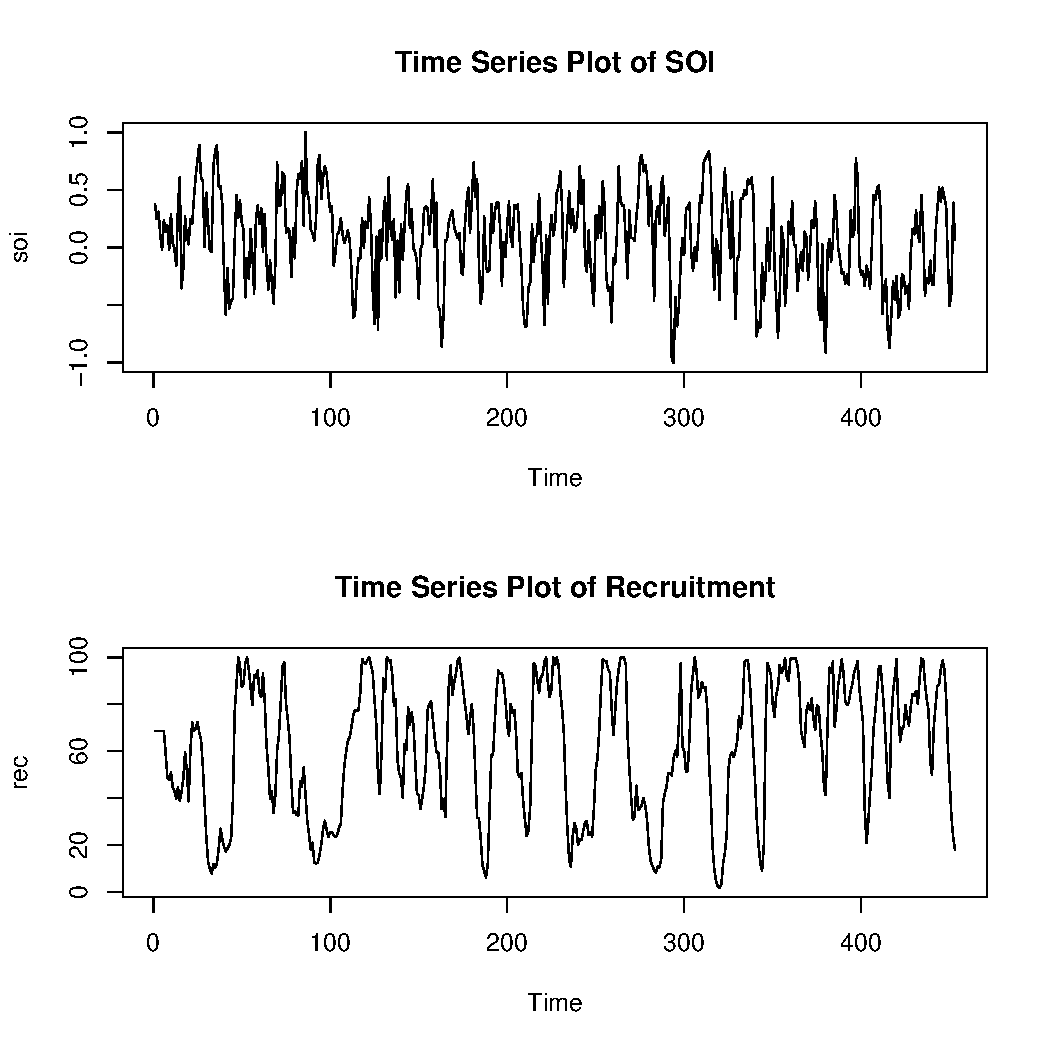
\includegraphics[width=110mm, height=55mm]{ts.pdf}

Residuals appear to be curved (keep in mind). A quadratic term for the predictor should be considered.

\end{frame}

\begin{frame}
\frametitle{Worked Example: Sales}

\includegraphics[width=110mm, height=55mm]{acfs.pdf}

Residuals appear to have an AR(1) structure.

\end{frame}

\begin{frame}[fragile]
\frametitle{Worked Example: Sales}

\verb=sarima()= function in R from \verb=astsa= package carries out steps 3, 4, 5. 

\begin{verbatim}
> sarima(company, 1, 0, 0, xreg=cbind(industry))
\end{verbatim}


\end{frame}



\begin{frame}[fragile]
\frametitle{Worked Example: Sales}


\begin{verbatim}
          Estimate     SE t.value p.value
ar1         0.6295 0.1772  3.5531  0.0024
intercept  -1.2876 0.3523 -3.6549  0.0020
industry    0.1751 0.0024 73.3658  0.0000
\end{verbatim}


\end{frame}

\begin{frame}
\frametitle{Worked Example: Sales}


\includegraphics[width=110mm, height=75mm]{diag1.pdf}



\end{frame}

\begin{frame}
\frametitle{Worked Example: Sales}

So the model is

\vspace{50mm}

\end{frame}

\begin{frame}[fragile]
\frametitle{Worked Example: Sales}

Should try a model with a quadratic term for the predictor. Turns out the quadratic term is insignificant.



\end{frame}

\begin{frame}
\frametitle{Extension to ARMA Errors}

Suppose the errors follow an ARMA process such that

$$
\phi(B) x_t = \theta(B)w_t.
$$



\textbf{Question}: How do we transform (\ref{eq:classic})?

\end{frame}


\end{document} 